\chapter{Детали реализации и тестирование}
В данной главе будут описаны некоторые интересные детали реализации описанных ранее алгоритмов. Во многом аппаратная часть определила подходы, которые использовались при теоретическом исследовании. Все перечисленное было реализовано в виде программных сервисов на языке Java~8.
\section{Работа с базой данных}
Исходя из размера всей транспортной сети, в которую входит информация об узлах, рейсах и расписаниях, не сложно заметить, что её нельзя уместить целиком в оперативной памяти и поэтому нужно использовать эффективное хранение информации -- базу данных. В данной работе была использована VoltDB.
\subsection{Особенности базы данных}
VoltDB - это ACID-совместимая реляционная СУБД, которая использует архитектуру shared nothing architecture. Она опирается на:
\begin{itemize}
	\item горизонтальную разбивку данных (каждый кластер хранит только свою порцию данных) вплоть до отдельного аппаратного потока;
	\item синхронную репликацию данных между всеми обработчиками одного кластера (для обеспечения высокой доступности);
	\item сочетание непрерывных снимков и журнала выполненных команд для обеспечения надежности данных (при восстановлении после сбоя).
\end{itemize}
VoltDB является in-memory СУБД, то есть старается преимущественно держать данные в оперативной памяти сервера, такой подход имеет ряд преимуществ: резко сокращается время отклика и становится проще репликация данных.
\subsection{Персистентные модели данных}
К сожалению, VoltDB поддерживает не все возможности обычных SQL СУБД, поэтому для версионности моделей и хранения истории данных, работа с ней происходит в Key-Value подходе, где ключом является любой комбинированный объект, состоящих из примитивных типов, а значением -- сериализованный Java-объект. Вместо стандартной сериализации используется библиотека Protostuff, которая имеет больше возможностей по сжатию и эффективному хранению данных.

Так как база данных почти полностью написана на Java, хранит объекты Java и предоставляет драйвер на том же языке, то ради повышения производительности объекты стоит сделать персистетными (иммутабельными), чтобы исключить блокировки. Это позволит работать с базой множеству отдельных потоков, исключая траты ресурсов на синхронизацию. 
\subsubsection{Транспорт}
Каждая реальная модель данных разделяется на абстрактную модель Model, в которой хранятся данные, и сущность из базы данных Entity, в которой хранится идентификатор (ID) и номер версии. База данных позволяет работать с сущностями посредством получения текущей версии и изменения модели, которую можно записать в сущность с автоматическим поднятием версии. При этом объект может либо блокироваться на момент обновления, либо работать без блокировок и использовать обновление отдельных полей.
\subsubsection{Остановки и пересадки}
В данный момент нельзя не сказать про очень важное требование к системе -- каждое значение в базе данных не должно занимать больше 1 Мбайт, это исходит из ограничений на размер результата базы данных и особенностей её репликаций, таким образом оно сильно усложняет возможность хранения множеств $T_d(s)$ и $T_a(s)$, доступных по ключу $s$. На данном этапе требуемая память для 1 сущности:
\begin{table}[!h]
	\caption{Базовый расход памяти на 1 сущность.}\label{tab3}
	\centering
	\begin{tabu}{|*{3}{X[c]|}}\hline
		Количество остановок & Занимаемая память (Плотно), Мбайт & Занимаемая память (Нормально), Мбайт \\\hline
		100  & 0.052 & 0.04\\\hline
		1000  & 0.52 & 0.48\\\hline
		10000  & 5.27 & 4.84\\\hline
		100000  & 53.1 & 48.78\\\hline
	\end{tabu}
\end{table}

Плотным вариантом считаются некоторые вокзалы крупных городов, где временные промежутки между события прибытия и отбытия исчисляются в минутах. Для начала ради уменьшения памяти разделим элементарные остановки на 2 типа:
\begin{itemize}
	\item \textbf{Облегченные остановки}. Они будут храниться во множествах $T_d(s)$ и $T_a(s)$ и соответствовать событиям отправления и прибытия на станцию $s$. Содержать будут только номер и ссылку на транспортный рейс.
	\item \textbf{Полные остановки}. В момент получения облегченные остановки будут можно дополнить до полных, так как в тот момент уже будет известна станция и время.
\end{itemize}

\begin{table}[!h]
	\caption{Расход памяти на 1 сущность (Без дублирования)}\label{tab3}
	\centering
	\begin{tabu}{|*{3}{X[c]|}}\hline
		Количество остановок & Занимаемая память (Плотно), Мбайт & Занимаемая память (Нормально), Мбайт \\\hline
		100  & 0.04 & 0.04\\\hline
		1000  & 0.36 & 0.4\\\hline
		10000  & 3.68 & 4.08\\\hline
		100000  & 37.29 & 41.19\\\hline
	\end{tabu}
\end{table}

В данной работе оптимальным вариант решения этой проблемы оказалось разделение этих множеств на более мелкие. Рассмотрим подробнее, что из себя представляет, например, множество $T_d(s)$. В нем хранятся элементарные остановки, которые содержат номер, станцию, транспортный рейс и время. Учитывая, что рейсы повторяются на станции достаточно редко, то разобьем множества по времени. Для этого приведен время в нормализованный вид и переведем в номер. Например, можно из времени убрать часы, минуты и более мелкие величины, то есть извлечь только дату, а уже её перевести в unix-time\footnote{Определяется как количество секунд, прошедших с полуночи (00:00:00 UTC) 1 января 1970 года. В нашем случае можно уменьшить ещё в 3600 раз.}, который будет являться номером. Тогда все множества разобьются на страницы, которые будут хранить только часть элементарных облегченных остановок.

\begin{figure}[!h]
	\centering
	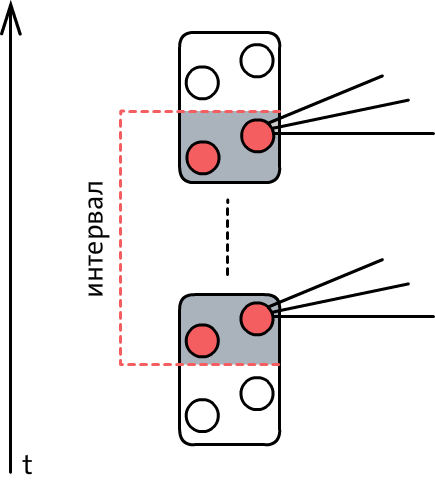
\includegraphics[width=0.5\textwidth]{schedule_pages.png}
	\caption{Страницы элементарных остановок с выходящими сегментами}\label{fig1}
\end{figure}

В результате ряда тестов и исследования методов сериализации в Java было обнаружено, что параметризованные сущности (Generics) сильно влияют на количество памяти после сериализациии. Таким образом, было решено полностью от них избавиться, прописав везде конкретные типы. Также пришлось отказаться от наиболее эффективной структуры данных для получения элементарных остановок в пределах указанного времени java.util.TreeMap, так как её стандартная реализация избыточно хранит большое количество ссылок, а также не поддерживает хранение множества значений для одного ключа (несколько поездов могут отбыть или прибыть в одно и тоже время с точностью до минуты). Наиболее компактной структурной для хранения одной страницы элементарных остановок оказался обычный java.util.ArrayList для пар время-остановка.

\begin{table}[!h]
	\caption{Оптимизированный расход памяти на 1 сущность.}\label{tab3}
	\centering
	\begin{tabu}{|*{3}{X[c]|}}\hline
		Количество остановок & Занимаемая память (Плотно), Мбайт & Занимаемая память (Нормально), Мбайт \\\hline
		100  & 0.01 & 0.01\\\hline
		1000  & 0.07 & 0.08\\\hline
		10000  & 0.71 & 0.87\\\hline
		100000  & 7.14 & 8.69\\\hline
	\end{tabu}
\end{table}

В результате мы может сохранять до 10000 остановок на одну страницу, этого достаточно для всех крупных вокзалов. Обновление страниц будет происходить не часто, поэтому его можно производить с полным копированием данных каждой обновляемой страницы.
\subsection{Кэши}
Зачем это нужно? Конечная система или построитель маршрутов будет географически распределен, база данных будет почти всегда находится физически в другом месте, а требоваться модели будут с различной регулярностью и актуальностью. Поэтому в построитель маршрутов будет добавлено несколько видов кэшей для ускорения работы.

Во-первых, мы добавим кэш для моделей данных. В нем для каждого типа объекта будет храниться его срок годности или частота, с которой его следует обновлять напрямую из базы данных.

Во-вторых, будет добавлен кэш для запросов $q = (s_d, t_d, s_a, t_a, k)$, где для каждого запроса $q$ будет сформирован на основе $s_d$ и $s_a$ уникальный ID, по которому можно будет сохранять результат фазы обхода, то есть множества сегментов и состояний построения. К сожалению, объем памяти построителя маршрутов и клиентского приложения сильно ограничены (для серверной конфигурации), поэтому кэш нужно ограничить по количеству запросов или памяти. Для такой задачи прекрасно подойдет LRU-кэш, то есть кэш основанный на алгоритме кэширования, при котором происходит вытеснение давно неиспользуемых запросов.
\section{Генерация карт транспортных сетей}
Для сравнения и тестирования различных алгоритмов построения маршрутов требуются данные. К сожалению, невозможно выгрузить реальные данные из закрытой системы, а также запустить на идентичных данных разные алгоритмы (данные постоянно меняются), поэтому для тестирования понадобятся дополнительные инструменты. Одним из таким инструментов будет процедурный генератор естественных транспортных сетей.

\begin{figure}[!h]
	\centering
	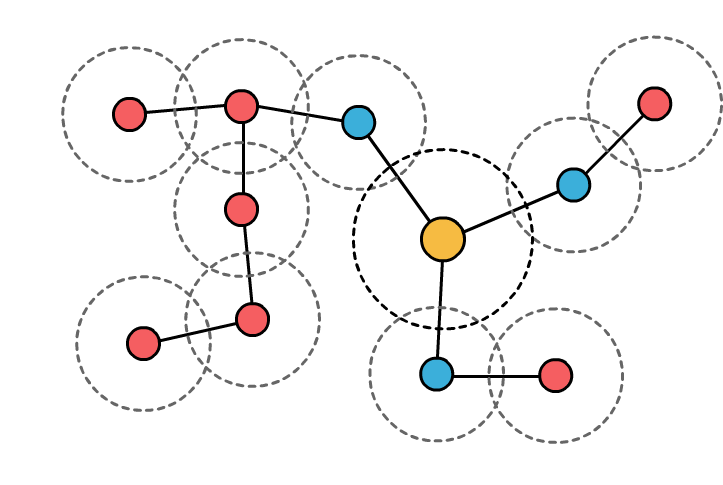
\includegraphics[width=0.9\textwidth]{transport_network.png}
	\caption{Сгенерированная абстрактная транспортная сеть с 1 городом и 3 вокзалами.}\label{fig1}
\end{figure}

Первым делом сгенерируем координаты транспортных узлов. В данном случае можно воспользоваться обычным равномерным псевдослучайным генератором чисел в области ограниченной некоторой кривой. Далее случайным образом выбираются типы транспортных узлов и их признаки из доступного множества признаков.

\subsection{Генерация транспортных рейсов}
Прокладка естественных маршрутов.
\subsection{Генерация центральных узлов}
Генерация точек-городов.

\FloatBarrier
\section{Результаты тестирования}
Время запроса с 10с до 2с, прикрепить 3 графика. Сравнение со старой системой, сравнение с Йеном.

\chapterconclusion
Все сделано и работает. Скорость работы возросла, новые функции появились. Покрыто интеграционными и авто тестами.
